\section{Resultados}\label{sec:resultados}
A continuación, se presentan los casos de estudio que se han realizado para diferentes simulaciones del juego
de la vida en dos y tres dimensiones, y sus respectivos resultados.
Para cada caso, se detallan los parámetros de entrada fijos utilizados, seguido de una o más figuras en el que
se muestra la evolución del sistema en cada paso temporal en valores extremos, y finalmente, un análisis del
observable en función de la densidad de celdas vivas en el dominio inicial.

\subsection{Conway en 2D}\label{subsec:conway-en-2d}

Como primer modelo, se ha estudiado el reconocido juego de la vida de Conway en dos dimensiones.
Para ello, se fija los siguientes parámetros de entrada:

\begin{itemize}
    \item $border = (0, 0) \times (100, 100)$
    \item $condition = MOORE$
    \item $r = 1$
    \item $shouldKeepAlive = [2, 3]$
    \item $shouldRevive = [3]$
    \item $initialDomainProportion = 0.16$
\end{itemize}
Variando el parámetro $initialLiveCellsProportion$ entre 0.1 y 0.9, se ha analizado la cantidad de celdas vivas
a lo largo de los pasos temporales.
\begin{figure}[H]
    \centering
    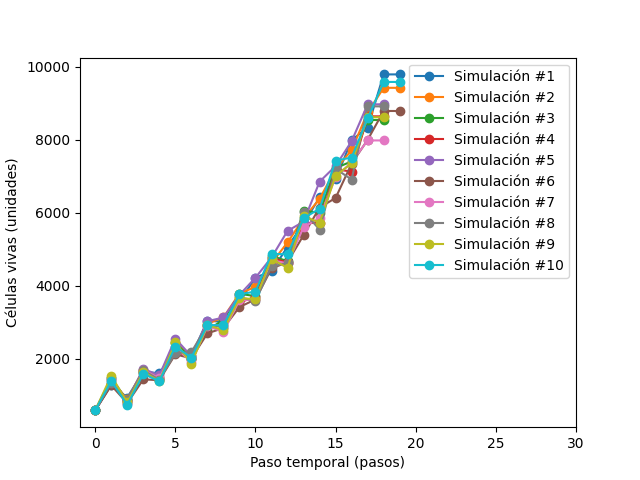
\includegraphics[width=0.6\linewidth]{conway2d/size_i10}
    \caption{Evolución en el tiempo del sistema de Conway con $initialLiveCellsProportion = 0.1$}
    \label{fig:conway2d_i10}
\end{figure}
\begin{figure}[H]
    \centering
    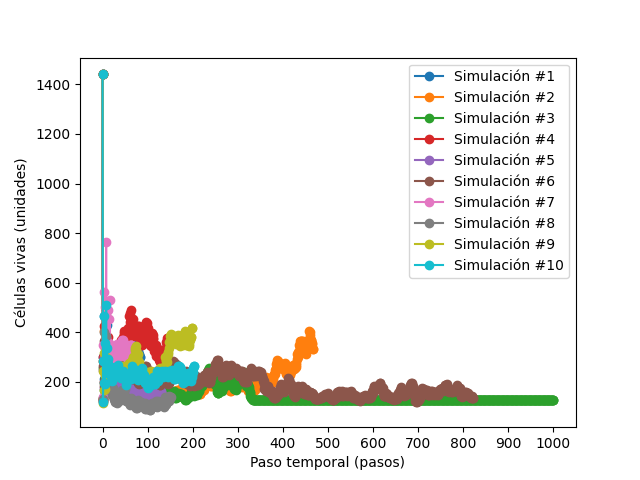
\includegraphics[width=0.6\linewidth]{conway2d/size_i90}
    \caption{Evolución en el tiempo del sistema de Conway con $initialLiveCellsProportion = 0.9$}
    \label{fig:conway2d_i90}
\end{figure}